% This LaTeX was auto-generated from MATLAB code.
% To make changes, update the MATLAB code and export to LaTeX again.

\documentclass{article}

\usepackage[utf8]{inputenc}
\usepackage[T1]{fontenc}
\usepackage{lmodern}
\usepackage{graphicx}
\usepackage{color}
\usepackage{hyperref}
\usepackage{amsmath}
\usepackage{amsfonts}
\usepackage{epstopdf}
\usepackage[table]{xcolor}
\usepackage{matlab}

\sloppy
\epstopdfsetup{outdir=./}
\graphicspath{ {./uloha1_gebhart_hurdzan_images/} }

\begin{document}

\matlabtitle{Úloha 1. FREKVENČNÍ FILTR}

\begin{par}
\begin{flushleft}
TPŘRS 2022
\end{flushleft}
\end{par}

\begin{par}
\begin{flushleft}
Skupina: 4 (\textbf{B1 HP})
\end{flushleft}
\end{par}

\begin{par}
\begin{flushleft}
Vypracoval: Jan Gebhart, Tomáš Hurdzan
\end{flushleft}
\end{par}

\begin{par}
\begin{flushleft}
Dne: 9.3.2022
\end{flushleft}
\end{par}


\vspace{1em}
\matlabheadingtwo{1. Navrhněte co nejednoudušší přenosovou funkci frekvečního filtru typu horní propust dle prototypu Čebyšev I, která bude vyhovovat nýsledujícím mezím:}

\begin{matlabcode}
%% Zadané hodnoty

% Zakázaná oblast "_p" jako passband
% f_p je zároveň, mezní frekvence (pro F_p = -3dB)
f_p = 1000; % maximalní frekvence propustneho pasma [Hz]
% omega_p je zároveň, mezní uhlová rychlost (pro F_p = -3dB)
omega_p = f_p * 2*pi; % maximalní uhlová rychlost propustneho pasma [rad/s]
F_p = -3; % maximalní hodnota útlumo propustného pásma |F_p| [dB]

% Zakázaná oblast "_s" jako Stopband
f_s = 250; % mezní frekvence [Hz]
omega_s = f_s * 2*pi; % mezní úhlová rychlost [rad/s]
F_s = -20; % mezní přenos |F_s| [dB]
%F(∞)= 0 dB

% meze grafů
xMin=1E2;
xMax=1E6;
yMin=-50;
yMax=10;

% body pro vykresleni charakteristik
omega_logspace=logspace(log10(xMin),log10(xMax),100);
\end{matlabcode}


\begin{matlabcode}
% bod 1
R_p=3; % překmit
[n,Wp] = cheb1ord(omega_p,omega_s, R_p, abs(F_s),"s");

fprintf("Mimimální počet pólů je %d", n);
\end{matlabcode}
\begin{matlaboutput}
Mimimální počet pólů je 2
\end{matlaboutput}
\begin{matlabcode}
[z,p,k] = cheb1ap(n,R_p);

% vypočteme přenos pro zesílení 1
[num,den] = zp2tf(z,p,1);
% dosadime nulovou frekvenci a vypocteme utlum
k2=den(end)/num(end);
% posunuti o velikost překmitu
k3 = k*10^(R_p/20);
% mohu použít k2 nebo k3
[num_tmp,den_tmp] = zp2tf(z,p,k3);
\end{matlabcode}


\begin{matlabcode}
% Mezní frekvence pro Chebyshev neodpovídá utlumu o 3 dB viz
% https://en.wikipedia.org/wiki/Cutoff_frequency

%% metoda půlení intervalu
mag_cheb=10^(-3/20); %požadované zesílení
mag_tmp=0;
omega_a=omega_p*0.5;
omega_b=omega_p*1.5;
omega_tmp=omega_p;
while abs(mag_tmp-mag_cheb)>1E-10
    [num,den] = lp2hp(num_tmp,den_tmp,omega_tmp);
    [mag_tmp]=bode(tf(num,den),omega_p);
    if mag_tmp-mag_cheb>0
        omega_a=omega_tmp;
    else
        omega_b=omega_tmp;
    end
    omega_tmp=(omega_a+omega_b)/2;
end
mag_tmp
\end{matlabcode}
\begin{matlaboutput}
mag_tmp = 0.7079
\end{matlaboutput}
\begin{matlabcode}
omega_tmp
\end{matlabcode}
\begin{matlaboutput}
omega_tmp = 7.3418e+03
\end{matlaboutput}


\begin{matlabcode}
[num,den] = lp2hp(num_tmp,den_tmp,omega_tmp);

F_cheb = tf(num,den) % vypoceteny prenos
\end{matlabcode}
\begin{matlaboutput}
F_cheb =
 
  s^2 + 1.286e-12 s + 1.889e-08
  -----------------------------
     s^2 + 6688 s + 7.614e07
 
Continuous-time transfer function.
\end{matlaboutput}
\begin{matlabcode}

[mag_cheb,phase_cheb]=bode(F_cheb,omega_logspace); %,

% "a" je zisk/utlum "A" je přenos
a_cheb=20*log10(mag_cheb(:));


% ==========================graf======================
figure;
axes("XScale","log");
hold on;
grid on;
legend("show","Location","southeast");
xlabel("omega [rad/s]");
ylabel("A [dB]");
axis([xMin xMax yMin yMax])
x = [xMin omega_s omega_s xMin];
y = [F_s F_s yMax yMax];
patch(x,y,"yellow","DisplayName","Stopband");
x = [xMax omega_p omega_p xMax];
y = [F_p F_p yMin yMin];
patch(x,y,"blue","DisplayName","Passband");
%====================================================
title("Útlumová frekvenční charakteristika");
plot(omega_logspace,a_cheb,"DisplayName","Chebyshev")
exportgraphics(gca,'twoplots.eps')
\end{matlabcode}
\begin{center}
\includegraphics[width=\maxwidth{56.196688409433015em}]{figure_0.eps}
\end{center}

\matlabheadingtwo{2. V rámci yadaného schématu určete hodnty obecných dvojpólů aktivní RC operační sítě}

\begin{par}
\begin{flushleft}
\includegraphics[width=\maxwidth{35.82538886101355em}]{image_0}
\end{flushleft}
\end{par}

\begin{matlabcode}
% bod 2
% ze zadaní
C = 33.2 * 10^-9 ;

[num, den] = tfdata(F_cheb);

% koeficienty viz přednáška
k0 = num{1}(1);
k1 = den{1}(3);
k2 = den{1}(2);

% vypoctene hodnoty _t
% viz prednasky
R1_t = k2 / (k1* 2 * C);
R2_t = 2/(k2 * C);
R3_t = 0;
R4_t = inf;
C1_t=C;
C2_t=C;

fprintf("Teoretická hodnota R1 = %f [ohm]",R1_t);
\end{matlabcode}
\begin{matlaboutput}
Teoretická hodnota R1 = 1322.889531 [ohm]
\end{matlaboutput}
\begin{matlabcode}
fprintf("Teoretická hodnota R2 = %f [ohm]",R2_t);
\end{matlabcode}
\begin{matlaboutput}
Teoretická hodnota R2 = 9007.422016 [ohm]
\end{matlaboutput}
\begin{matlabcode}
fprintf("Teoretická hodnota R3 = %f [ohm]",R3_t);
\end{matlabcode}
\begin{matlaboutput}
Teoretická hodnota R3 = 0.000000 [ohm]
\end{matlaboutput}
\begin{matlabcode}
fprintf("Teoretická hodnota R4 = %f [ohm]",R4_t);
\end{matlabcode}
\begin{matlaboutput}
Teoretická hodnota R4 = Inf [ohm]
\end{matlaboutput}
\begin{matlabcode}
fprintf("Teoretická hodnota C1 = %f [ohm]",C1_t);
\end{matlabcode}
\begin{matlaboutput}
Teoretická hodnota C1 = 0.000000 [ohm]
\end{matlaboutput}
\begin{matlabcode}
fprintf("Teoretická hodnota C2 = %f [ohm]",C2_t);
\end{matlabcode}
\begin{matlaboutput}
Teoretická hodnota C2 = 0.000000 [ohm]
\end{matlaboutput}

\matlabheadingtwo{3. Určete typy a hodnoty pasivních dvojpólů pasivního RC článku, stejného typu a mezní frekvecí jako u aktivní sítě}

\begin{matlabcode}
% bod 3
C0_t=C;
% viz prednasky
R0_t = 1/(omega_p*C0_t);
fprintf("Teoretická hodnota R0 = %f [ohm]",R0_t);
\end{matlabcode}
\begin{matlaboutput}
Teoretická hodnota R0 = 4793.823587 [ohm]
\end{matlaboutput}

\matlabheadingtwo{4. Odvoďte a spočtěte frekvenční přenos navrženého obvodového řešení filtru (bez i s přídavným RC článkem). Porovnejte logaritmické frekvenční charakteristiky spočtených přenosů s frekvenčními charakteristikami navržených teoretických přenosů.}

\begin{matlabcode}
% hodnoty skutecnych soucastek
C0_s= 33.63 * 10^-9;
C1_s = 33.97 * 10^-9;
C2_s = 33.45 * 10^-9;

R0_s = 4.7251 * 10^3;
R1_s = 1.284 * 10^3;
R2_s = 8.799 * 10^3;
\end{matlabcode}


\begin{par}
\begin{flushleft}
Teoretický přenos Chebyshevova filtru je:
\end{flushleft}
\end{par}

\begin{matlabcode}
% bod 4 bez RC
% teoreticky
num = [C1_t*C2_t*1, 0 , 0];
den = [C1_t*C2_t, (C1_t+C2_t)/R2_t - 0 , 1/(R1_t*R2_t)];
F_cheb_t=tf(num,den)
\end{matlabcode}
\begin{matlaboutput}
F_cheb_t =
 
               1.102e-15 s^2
  ---------------------------------------
  1.102e-15 s^2 + 7.372e-12 s + 8.392e-08
 
Continuous-time transfer function.
\end{matlaboutput}
\begin{matlabcode}
[mag_cheb_t,phase_cheb_t]=bode(F_cheb_t,omega_logspace);
a_cheb_t=20*log10(mag_cheb_t(:));

\end{matlabcode}

\begin{par}
\begin{flushleft}
Skutečný přenos Chebyshevova filtru je:
\end{flushleft}
\end{par}

\begin{matlabcode}
% skutecne
num = [C1_s*C2_s*1, 0 , 0];
den = [C1_s*C2_s, (C1_s+C2_s)/R2_s - 0 , 1/(R1_s*R2_s)];
F_cheb_s=tf(num,den)
\end{matlabcode}
\begin{matlaboutput}
F_cheb_s =
 
               1.136e-15 s^2
  ---------------------------------------
  1.136e-15 s^2 + 7.662e-12 s + 8.851e-08
 
Continuous-time transfer function.
\end{matlaboutput}
\begin{matlabcode}
[mag_cheb_s,phase_cheb_s]=bode(F_cheb_s,omega_logspace);
a_cheb_s=20*log10(mag_cheb_s(:));


% ==========================graf======================
figure;
subplot(2,1,1,"XScale","log");
hold on;
grid on;
legend("show","Location","southeast");
xlabel("omega [rad/s]");
ylabel("A [dB]");
axis([xMin xMax yMin yMax])
x = [xMin omega_s omega_s xMin];
y = [F_s F_s yMax yMax];
patch(x,y,"yellow","DisplayName","Stopband");
x = [xMax omega_p omega_p xMax];
y = [F_p F_p yMin yMin];
patch(x,y,"blue","DisplayName","Passband");
title("Útlumová frekvenční charakteristika bez RC");
plot(omega_logspace,a_cheb_t,"DisplayName","Chebyshev teoreticky")
plot(omega_logspace,a_cheb_s,"DisplayName","Chebyshev skutecne")

subplot(2,1,2,"XScale","log");
hold on;
grid on;
legend("show","Location","east");
xlabel("omega [rad/s]");
ylabel("phase [°]");
title("Fáyová frekvenční charakteristika bez RC");
plot(omega_logspace,phase_cheb_t(:),"DisplayName","Chebyshev teoreticky")
plot(omega_logspace,phase_cheb_s(:),"DisplayName","Chebyshev skutecne")
\end{matlabcode}
\begin{center}
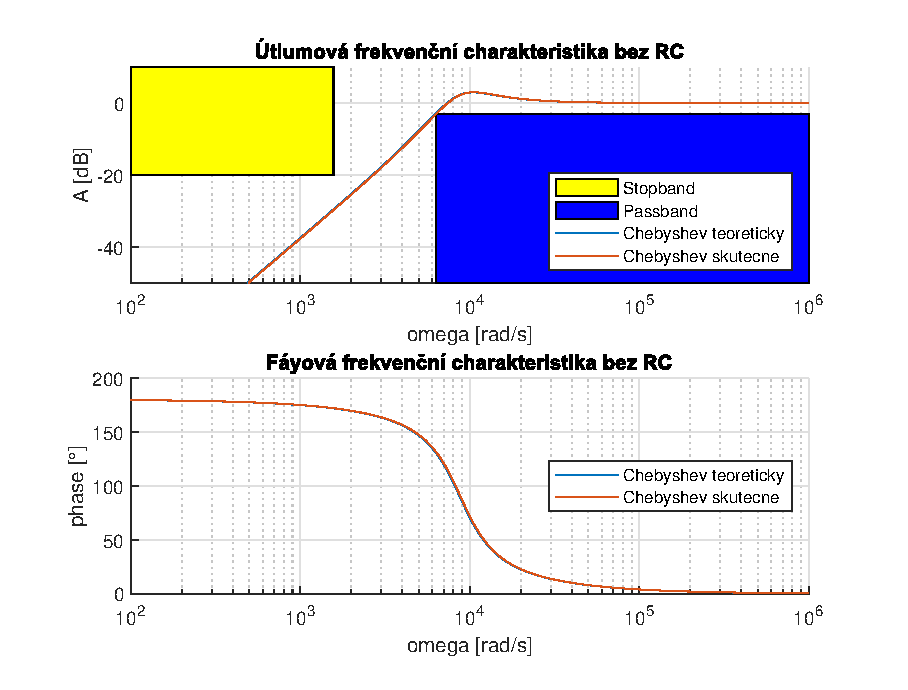
\includegraphics[width=\maxwidth{56.196688409433015em}]{figure_1.eps}
\end{center}
\begin{matlabcode}
%====================================================
\end{matlabcode}


\begin{matlabcode}
% bod 4 s RC
% z teoretickych hodnot
num = [(R0_t*C0_t)  0];
den = [(R0_t*C0_t) 1];
F_RC_t = tf(num, den);
F_cheb_rc_t = F_RC_t*F_cheb_t;
[mag_cheb_rc_t,phase_cheb_rc_t]=bode(F_cheb_rc_t,omega_logspace);
a_cheb_rc_t=20*log10(mag_cheb_rc_t(:));

% z skutecnych hodnot
num = [(R0_s*C0_s)  0];
den = [(R0_s*C0_s) 1];
F_RC_s = tf(num, den);
F_cheb_rc_s = F_RC_s*F_cheb_s;
[mag_cheb_rc_s,phase_cheb_rc_s]=bode(F_cheb_rc_s,omega_logspace);
a_cheb_rc_s=20*log10(mag_cheb_rc_s(:));


% ==========================graf======================
figure;
subplot(2,1,1,"XScale","log");
hold on;
grid on;
legend("show","Location","southeast");
xlabel("omega [rad/s]");
ylabel("A [dB]");
axis([xMin xMax yMin yMax])
x = [xMin omega_s omega_s xMin];
y = [F_s F_s yMax yMax];
patch(x,y,"yellow","DisplayName","Stopband");
x = [xMax omega_p omega_p xMax];
y = [F_p F_p yMin yMin];
patch(x,y,"blue","DisplayName","Passband");
title("Útlumová frekvenční charakteristika s RC");
plot(omega_logspace,a_cheb_rc_t,"DisplayName","Chebyshev s RC teoreticky")
plot(omega_logspace,a_cheb_rc_s,"DisplayName","Chebyshev s RC skutecne")


subplot(2,1,2,"XScale","log");
hold on;
grid on;
legend("show","Location","east");
xlabel("omega [rad/s]");
ylabel("phase [°]");
title("Fáyová frekvenční charakteristika s RC");
plot(omega_logspace,phase_cheb_rc_t(:),"DisplayName","Chebyshev s RC teoreticky")
plot(omega_logspace,phase_cheb_rc_s(:),"DisplayName","Chebyshev s RC skutecne")
\end{matlabcode}
\begin{center}
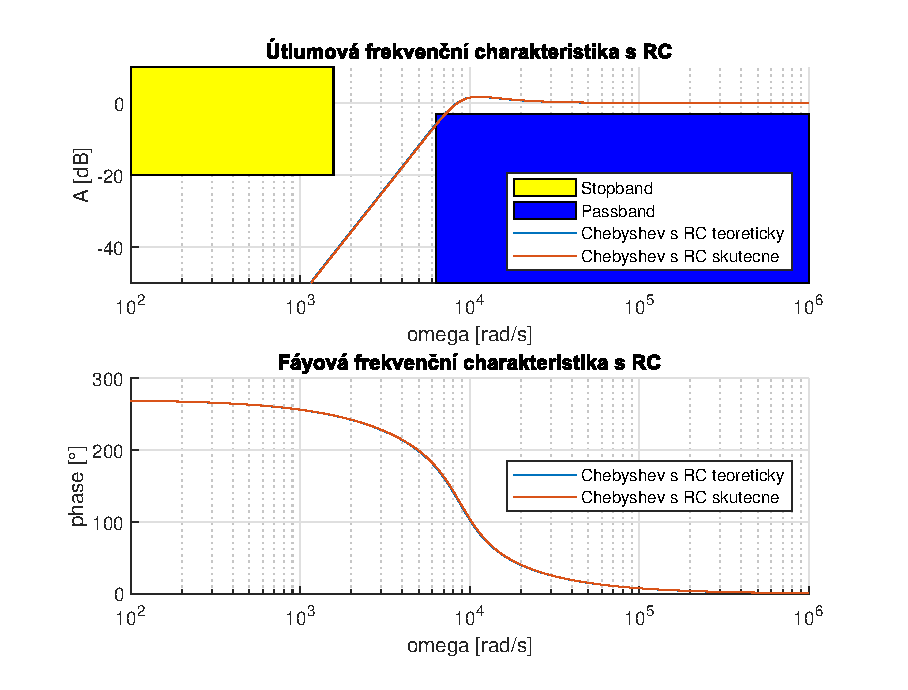
\includegraphics[width=\maxwidth{56.196688409433015em}]{figure_2.eps}
\end{center}
\begin{matlabcode}
%====================================================
\end{matlabcode}

\matlabheadingtwo{5. Realizujte obvodová řešení na částečně univerzální desce plošných spojů. Potřebné hodnoty součástek sestavte sériově-paralelní kombinací standardizovaných hodnot R a C. Výsledné hodnoty ověřte měřením vybraných součástek.}

\begin{matlabcode}
% bod 5
fprintf("Chyba R0 = %f %%",abs((R0_t-R0_s)/R0_s)*100);
\end{matlabcode}
\begin{matlaboutput}
Chyba R0 = 1.454437 %
\end{matlaboutput}
\begin{matlabcode}
fprintf("Chyba R1 = %f %%",abs((R1_t-R1_s)/R1_s)*100);
\end{matlabcode}
\begin{matlaboutput}
Chyba R1 = 3.028780 %
\end{matlaboutput}
\begin{matlabcode}
fprintf("Chyba R2 = %f %%",abs((R2_t-R2_s)/R2_s)*100);
\end{matlabcode}
\begin{matlaboutput}
Chyba R2 = 2.368701 %
\end{matlaboutput}
\begin{matlabcode}
fprintf("Chyba C0 = %f %%",abs((C0_t-C0_s)/C0_s)*100);
\end{matlabcode}
\begin{matlaboutput}
Chyba C0 = 1.278620 %
\end{matlaboutput}
\begin{matlabcode}
fprintf("Chyba C1 = %f %%",abs((C1_t-C1_s)/C1_s)*100);
\end{matlabcode}
\begin{matlaboutput}
Chyba C1 = 2.266706 %
\end{matlaboutput}
\begin{matlabcode}
fprintf("Chyba C2 = %f %%",abs((C2_t-C2_s)/C2_s)*100);
\end{matlabcode}
\begin{matlaboutput}
Chyba C2 = 0.747384 %
\end{matlaboutput}


\matlabheading{6. Změřte logaritmickou amplitudovou frekvenční charakteristiku filtru (bez i s přídavným RC článkem) metodou postupného měření amplitudy procházejícího sinusového signálu s proměnnou frekvencí. Frekvence volte v rozsahu 50 Hz — 20 kHz v logaritmické řadě s preferencí okolí omega\_p. Porovnejte naměřené frekvenční charakteristiky obou variant s charakteristikami z předchozích bodů.}

\begin{matlabcode}
% ociloskop data _o
f_o = [50 100 200 500 800 900 1000 1100 1200 1500 2000 5000 10000 20000];
omega_logspace_o = f_o*2*pi;
U2_cheb_o = [32*10^-3 36*10^-3 56*10^-3 272*10^-3 880*10^-3 1.1 1.35 1.67 1.99 2.73 2.73 2.13 2.05 2.05];
U2_cheb_rc_o = [0*10^-3 0*10^-3 23*10^-3 93*10^-3 280*10^-3 370*10^-3 480*10^-3 680*10^-3 800*10^-3 1.16 1.89 2.13 2.05 2.01];
U1_o = 2;
\end{matlabcode}


\begin{matlabcode}
% bod 6 bez RC
A_cheb_o=U2_cheb_o/U1_o;
a_cheb_o=20*log10(A_cheb_o);

% ==========================graf======================
figure;
utlumova_charakteristika=axes("XScale","log");
hold on;
grid on;
legend("show","Location","southeast");
xlabel("omega [rad/s]");
ylabel("A [dB]");
axis([xMin xMax yMin yMax])
x = [xMin omega_s omega_s xMin];
y = [F_s F_s yMax yMax];
patch(x,y,"yellow","DisplayName","Stopband");
x = [xMax omega_p omega_p xMax];
y = [F_p F_p yMin yMin];
patch(x,y,"blue","DisplayName","Passband");
title("Útlumová frekvenční charakteristika bez RC");
plot(omega_logspace,a_cheb_t,"DisplayName","Chebyshev teoreticky")
plot(omega_logspace,a_cheb_s,"DisplayName","Chebyshev skutecne")
plot(omega_logspace_o,a_cheb_o,"DisplayName","Chebyshev ociloskop")
\end{matlabcode}
\begin{center}
\includegraphics[width=\maxwidth{56.196688409433015em}]{figure_3.eps}
\end{center}
\begin{matlabcode}
%====================================================
\end{matlabcode}


\begin{matlabcode}
% bod 6 s RC
A_cheb_rc_o=U2_cheb_rc_o/U1_o;
a_cheb_rc_o=20*log10(A_cheb_rc_o);

% ==========================graf======================
figure;
utlumova_charakteristika_rc=axes("XScale","log");
hold on;
grid on;
legend("show","Location","southeast");
xlabel("omega [rad/s]");
ylabel("A [dB]");
axis([xMin xMax yMin yMax])
x = [xMin omega_s omega_s xMin];
y = [F_s F_s yMax yMax];
patch(x,y,"yellow","DisplayName","Stopband");
x = [xMax omega_p omega_p xMax];
y = [F_p F_p yMin yMin];
patch(x,y,"blue","DisplayName","Passband");
title("Útlumová frekvenční charakteristika s RC");
title("Útlumová frekvenční charakteristika s RC");
plot(omega_logspace,a_cheb_rc_t,"DisplayName","Chebyshev s RC teoreticky")
plot(omega_logspace,a_cheb_rc_s,"DisplayName","Chebyshev s RC skutecne")
plot(omega_logspace_o,a_cheb_rc_o,"DisplayName","Chebyshev s RC ociloskop")
\end{matlabcode}
\begin{center}
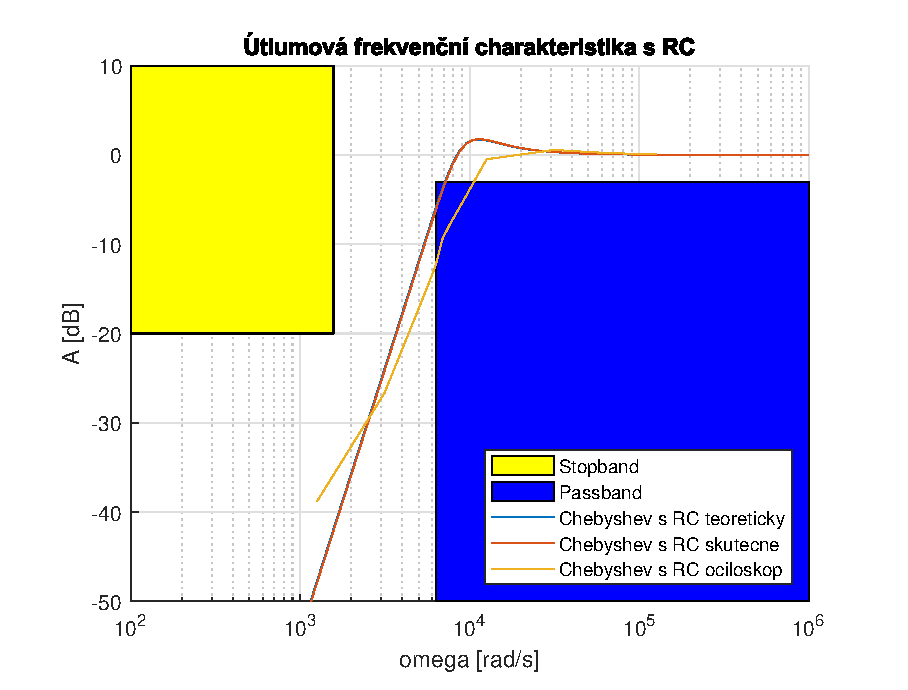
\includegraphics[width=\maxwidth{56.196688409433015em}]{figure_4.eps}
\end{center}
\begin{matlabcode}
%====================================================
\end{matlabcode}


\matlabheadingtwo{7. Změřte fázové zpoždění na frekvenci 1kHz. Porovnejte naměřené hodnoty obou variant s fáyovými charakteristikami z bodu 4.}

\begin{matlabcode}
% ociloskop hodnoty
omega_phase=1000*2*pi;
phase_cheb_o=130;
phase_cheb_rc_o=170;
\end{matlabcode}


\begin{matlabcode}
% bod 7 bez RC
figure;
subplot(2,1,1,"XScale","log");
hold on;
grid on;
legend("show","Location","east");
xlabel("omega [rad/s]");
ylabel("phase [°]");
title("Fázová frekvenční charakteristika bez RC");
scatter(omega_phase,phase_cheb_o,"DisplayName","Chebyshev ociloskop")
plot(omega_logspace,phase_cheb_t(:),"DisplayName","Chebyshev teoreticky")

% bod 7 s RC
subplot(2,1,2,"XScale","log");
hold on;
grid on;
legend("show","Location","east");
xlabel("omega [rad/s]");
ylabel("phase [°]");
title("Fázová frekvenční charakteristika s RC");
scatter(omega_phase,phase_cheb_rc_o,"DisplayName","Chebyshev s RC ociloskop")
plot(omega_logspace,phase_cheb_rc_t(:),"DisplayName","Chebyshev s RC teoreticky")
\end{matlabcode}
\begin{center}
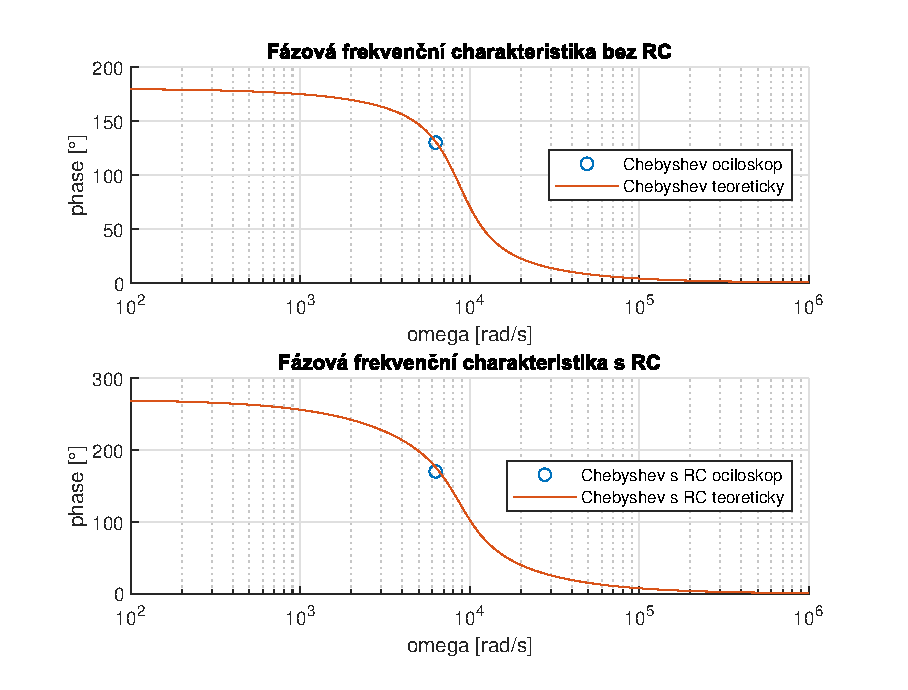
\includegraphics[width=\maxwidth{56.196688409433015em}]{figure_5.eps}
\end{center}

\matlabheadingtwo{8. Přeskočeno}

\matlabheadingtwo{9. Změřte logaritmickou amplitudovou frekvenční charakteristiku filtru (bez is přídavným RC článkem) metodou poměru amplitudových spekter výstupního signálu a vstupního signálu typu bílý šum. Porovnejte naměřené frekvenčni charakteristiky obou variant s charakteristikami přenosů z předchozích bodů.}


\begin{matlabcode}
% načtení dat bod 9 a 10
% prní slupec je casova značka, druhý slupec je generovaný výstup (vstup
% filtru), třetí slupec je měření vstupu filtru a čtvtý je měření výstupu
% mezi druhým a třetím slupcem je jednokrokove zpoždění

% Z naměřených dat budeme potrebovat 3. a 4. slupec (vstup a výstu filtru)
% Prvních 50 vzorků vynechám pro ustálení přechodových dějů
if isfile("data.mat")
    load("data.mat")
else
    bily_cheb = readmatrix("bily.xlsx","Sheet","sheet1","Range","C50:D100050");
    bily_cheb_rc = readmatrix("bily_rc.xlsx","Sheet","sheet1","Range","C50:D100050");
    step_cheb = readmatrix("step.xlsx","Sheet","sheet1","Range","B50:D15000");
    step_cheb_rc = readmatrix("step_rc.xlsx","Sheet","sheet1","Range","B50:D15000");
    save("data","bily_cheb","bily_cheb_rc","step_cheb","step_cheb_rc");
end
frekvence_vzorkovani=50000;
\end{matlabcode}


\begin{matlabcode}
% bod 9 bez RC
vstup_cheb=bily_cheb(:,1);
vystup_cheb=bily_cheb(:,2);

window = hamming(1024); %vzorkovací okno

IN=zeros(1024,1);
OUT=zeros(1024,1);
i=1;
while (i+1024)<length(vstup_cheb)
    IN = IN + abs(fft(vstup_cheb(i:i+1023).*window));
    OUT = OUT + abs(fft(vystup_cheb(i:i+1023).*window));
    i = i +512;
end

a_cheb_fft=20*log10(OUT(1:513)) - 20*log10(IN(1:513)); % OUT/IN jako rozdíl logaritmu
omega_cheb_fft = (0:512)/512*frekvence_vzorkovani/2*2*pi;
% ==========================graf======================
plot(utlumova_charakteristika,omega_cheb_fft,a_cheb_fft,"DisplayName","Chebyshev fft")
\end{matlabcode}
\begin{center}
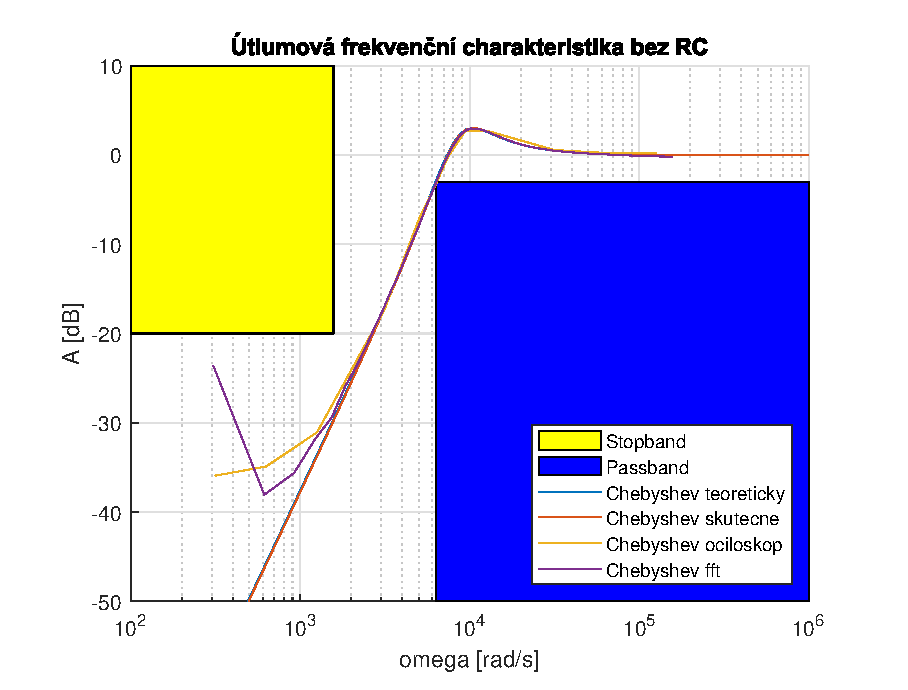
\includegraphics[width=\maxwidth{56.196688409433015em}]{figure_6.eps}
\end{center}
\begin{matlabcode}
%====================================================
\end{matlabcode}


\begin{matlabcode}
% bod 9 s RC
vstup_cheb=bily_cheb_rc(:,1);
vystup_cheb=bily_cheb_rc(:,2);

window = hamming(1024); %vzorkovací okno

IN=zeros(1024,1);
OUT=zeros(1024,1);
i=1;
while (i+1024)<length(vstup_cheb)
    IN = IN + abs(fft(vstup_cheb(i:i+1023).*window));
    OUT = OUT + abs(fft(vystup_cheb(i:i+1023).*window));
    i = i +512;
end

a_cheb_rc_fft=20*log10(OUT(1:513)) - 20*log10(IN(1:513)); % OUT/IN jako rozdíl logaritmu
omega_cheb_rc_fft = (0:512)/512*frekvence_vzorkovani/2*2*pi;
% ==========================graf======================
plot(utlumova_charakteristika_rc,omega_cheb_rc_fft,a_cheb_rc_fft,"DisplayName","Chebyshev s RC fft")
\end{matlabcode}
\begin{center}
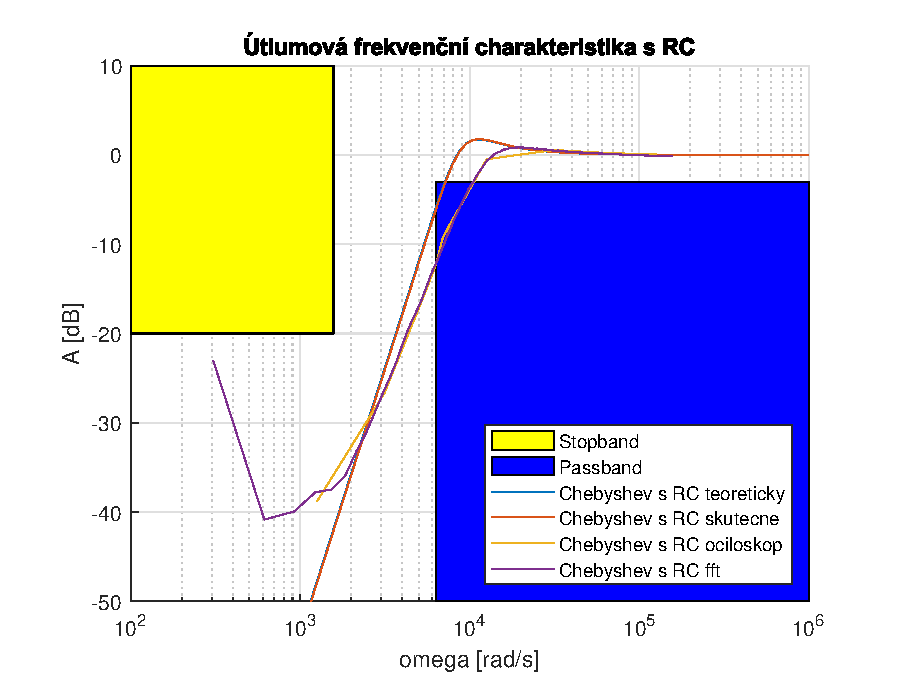
\includegraphics[width=\maxwidth{56.196688409433015em}]{figure_7.eps}
\end{center}
\begin{matlabcode}
%====================================================
\end{matlabcode}

\matlabheadingtwo{10. Změřte přechodovou ftrekvenční charakteristiku filtru (bez i s přídavným RC článkem) metodou vybuzení filtru napětovým skokem 0 -1 V. Porovnejte neměřené charakteristiky obou variant s přechodovýmí charakteristikami spočtených přenosů.}


\begin{matlabcode}
% data bod 10
perioda_vzorkovani=1/frekvence_vzorkovani;
doba_pro_vykresleni=0.003;
\end{matlabcode}


\begin{matlabcode}
% bod 10 bez RC
start=find(diff(step_cheb(:,1)))+1;
stop=start+floor(doba_pro_vykresleni/perioda_vzorkovani);

vystup_cheb=step_cheb(start:stop,3);
vstup_cheb=step_cheb(start:stop,2);

time_cheb=linspace(0,(length(vystup_cheb)-1)*perioda_vzorkovani,length(vystup_cheb));
[vystup_cheb_t,time_cheb_t]=step(F_cheb_t,doba_pro_vykresleni);

% ==========================graf======================
figure;
hold on;
grid on;
legend("show","Location","southeast");
xlabel("time [s]");
ylabel("amplitude [V]");

title("Přechodová charakteristika bez RC");
plot(time_cheb_t,vystup_cheb_t,"DisplayName","Chebyshev teoreticky");
plot(time_cheb,vystup_cheb,"DisplayName","Chebyshev namereny");
\end{matlabcode}
\begin{center}
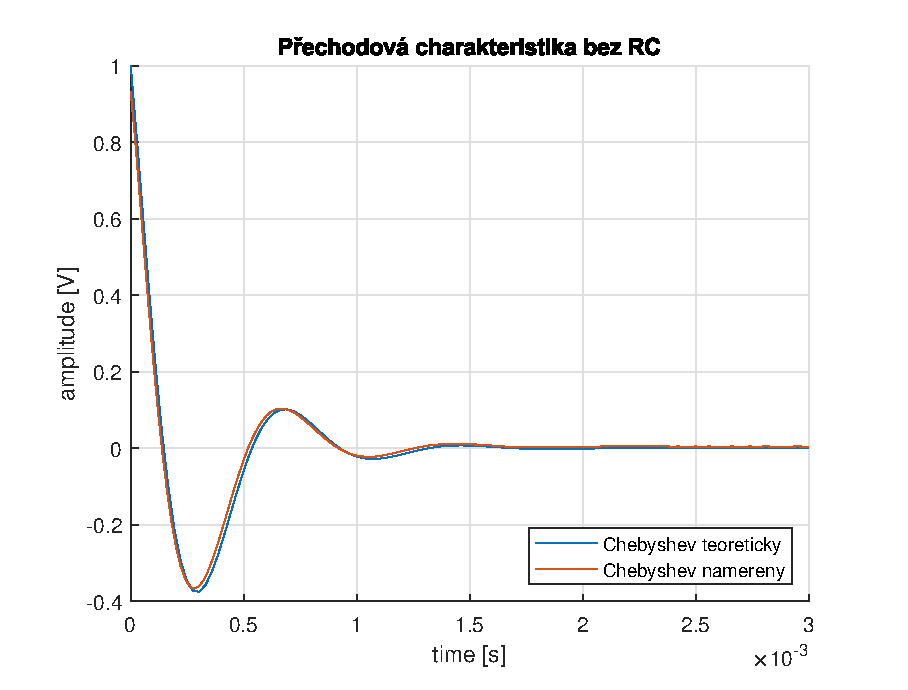
\includegraphics[width=\maxwidth{56.196688409433015em}]{figure_8.eps}
\end{center}
\begin{matlabcode}
%====================================================
\end{matlabcode}


\begin{matlabcode}
% bod 10 s RC
start=find(diff(step_cheb_rc(:,1)))+1;
stop=start+floor(doba_pro_vykresleni/perioda_vzorkovani);

vystup_cheb_rc=step_cheb_rc(start:stop,3);
vstup_cheb_rc=step_cheb_rc(start:stop,2);

time_cheb_rc=linspace(0,(length(vystup_cheb_rc)-1)*perioda_vzorkovani,length(vystup_cheb_rc));
[vystup_cheb_rc_t,time_cheb_rc_t]=step(F_cheb_rc_t,doba_pro_vykresleni);

% ==========================graf======================
figure;
hold on;
grid on;
legend("show","Location","southeast");
xlabel("time [s]");
ylabel("amplitude [V]");

title("Přechodová charakteristika s RC");
plot(time_cheb_rc_t,vystup_cheb_rc_t,"DisplayName","Chebyshev s RC teoreticky");
plot(time_cheb_rc,vystup_cheb_rc,"DisplayName","Chebyshev s RC namereny");
\end{matlabcode}
\begin{center}
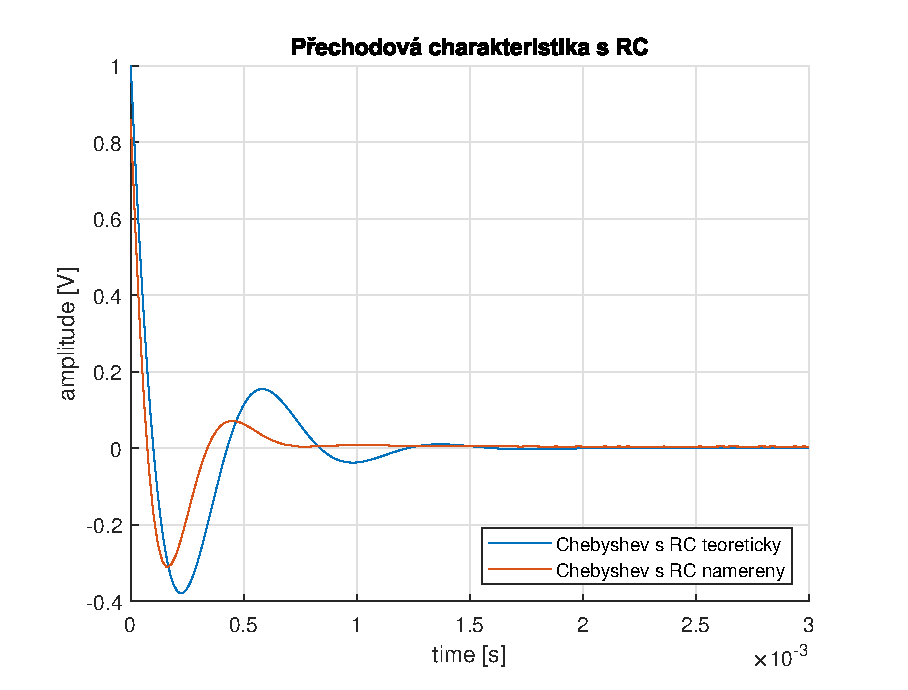
\includegraphics[width=\maxwidth{56.196688409433015em}]{figure_9.eps}
\end{center}
\begin{matlabcode}
%====================================================
\end{matlabcode}

\matlabheadingtwo{11. Závěr}

\begin{par}
\begin{flushleft}
TODO
\end{flushleft}
\end{par}

\end{document}
